%!TEX root = ../template.tex
%%%%%%%%%%%%%%%%%%%%%%%%%%%%%%%%%%%%%%%%%%%%%%%%%%%%%%%%%%%%%%%%%%%%
%% 3 - Elements.tex
%%   3.1 - 5G RAN
%%   3.2 - 5G Core
%%   3.3 - Existing 5G Packages for 5G Networks
%%   3.4 - Related Works  
%%%%%%%%%%%%%%%%%%%%%%%%%%%%%%%%%%%%%%%%%%%%%%%%%%%%%%%%%%%%%%%%%%%%
\graphicspath{{../5-Figures/}{5-Figures/}}
\chapter{Elements of a 5G Network}
\label{cha:elements_of_a_5g_network}
% Mention how 5G networks focus on modularity, where network functions expose their data to third parties. 
% Add a picture here of a 5G network architecture, showing the RAN and Core components.
% In this section, introduce the topic and talk about other projects that have implemented a 5G network using open-source packages, such as Open5GCube \cite{horstmann2025open5gcube}, 5GMap \cite{paci2025gmap}, and others \cite{mamushiane2023deploying, tio2025exploring5g}.

\section{Introduction to the 5G Architecture}
\label{sec:introduction_5g_architecture}
% Describe the evolution from 4G EPC to 5G NR, highlighting the service-based architecture, virtualization and cloud-native functions, network slicing and CUPS.
The 5G architecture represents a significant evolution from previous generations of mobile networks, particularly the 4G \gls{EPC}. Compared to the \gls{EPC}, the 5G architecture is designed to be more flexible, scalable, and efficient, enabling a wide range of novel use cases and services (see Figure~\ref{fig:5g_network_architecture}). 
\begin{figure}[H]
  \centering
  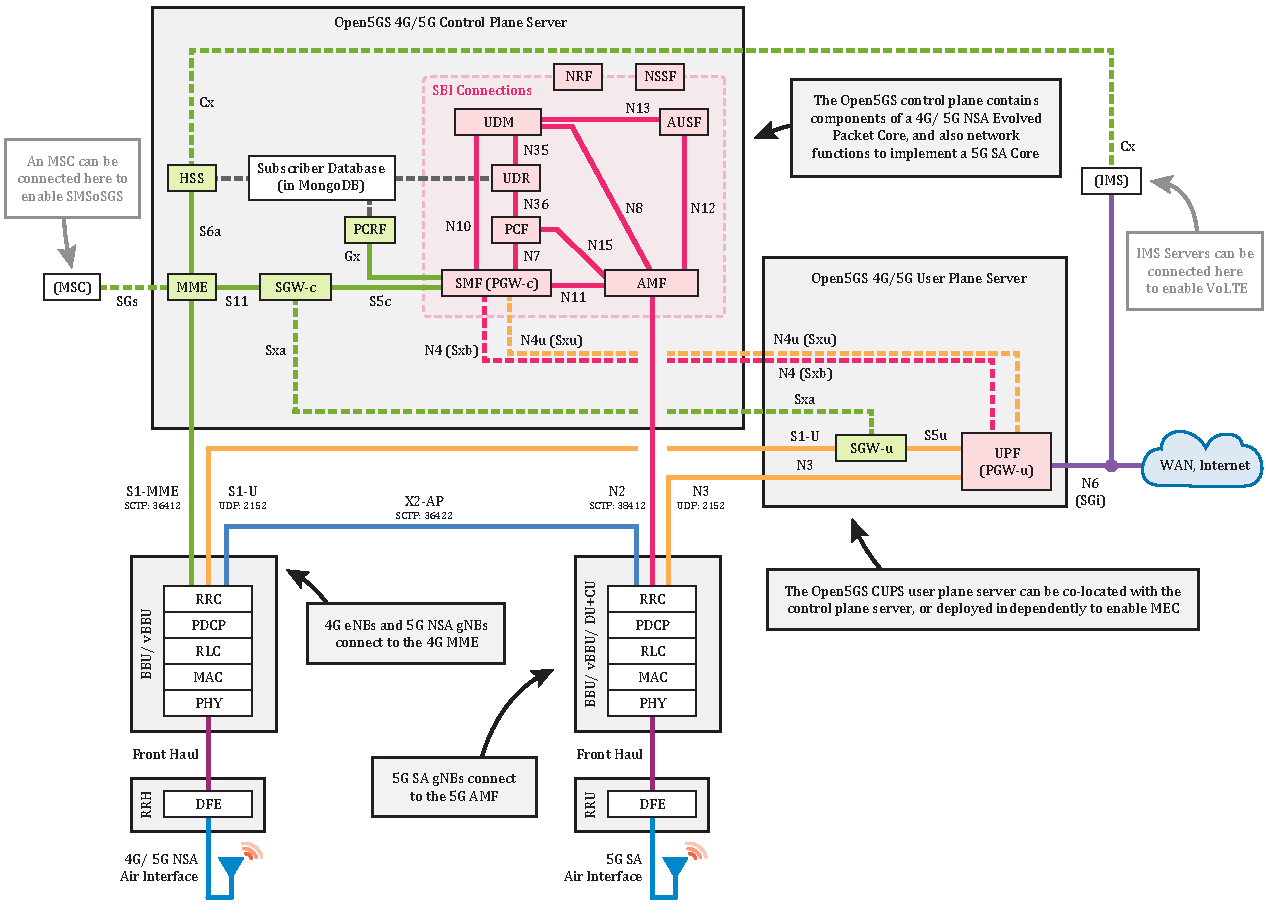
\includegraphics[width=\textwidth]{Open5GS_CUPS-01.pdf}
  \caption{\centering\small 5G Network architecture diagram from the Open5GS project~\cite{open5gs_repo}. Used under the AGPL-3.0 license.}
  \label{fig:5g_network_architecture}
\end{figure}

Key features of the 5G architecture include:    
\subsection*{\normalfont\uline{\glsxtrlong{SBA}}}
\label{sec:sba}
% Explain the SBA concept, NRF role importance, how services communicate via HTTP REST APIs, how they register, the roles of Service provider and consumer
Unlike the monolithic architecture of 4G and previous generations, 5G adopts a service-based approach where network functions are designed to be modular services that can be independently configured and implemented. Network functions expose their capabilities and communicate via HTTP/2, using a standardized REST API, allowing for interoperability between services.

In this paradigm, the functions take the roles of either Service Providers or Service Consumers, depending on whether they offer or utilize specific services. The \gls{NRF}, which will be developed upon further, plays a crucial role in this architecture by maintaining a registry of available network functions and their services, enabling dynamic discovery and interaction among them.

\subsection*{\normalfont\uline{\glsxtrlong{CUPS}}}
\label{sec:CUPS}

\begin{figure}[H]
  \centering
  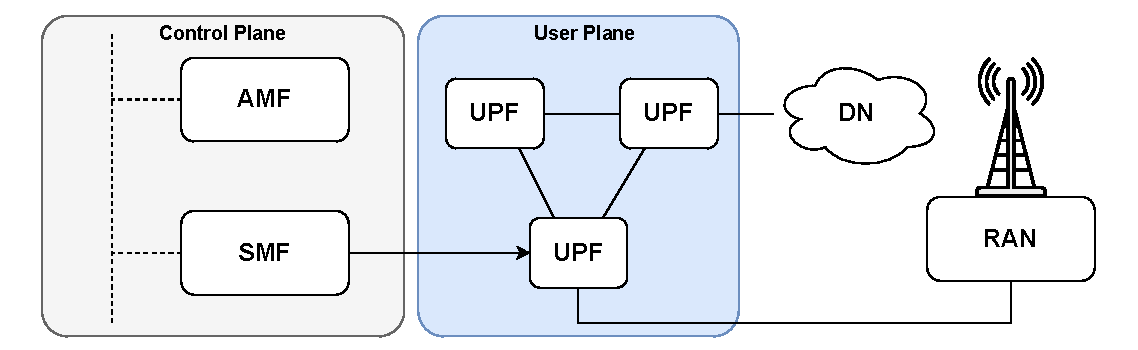
\includegraphics[width=0.9\textwidth]{5G CUPS.pdf}
  \caption{\centering\small Control and User Plane Separation.}
  \label{fig:CUPS}
\end{figure}
In 5G systems, the separation of the control plane and user plane is one of the fundamental design principles that sets them apart from previous generations, defining them as independent functional entities that can be deployed, scaled and managed separately, as shown on Figure~\ref{fig:CUPS}.

This means that network operators can dimension their networks to adapt to real network traffic patterns, deploying control plane functions in centralized locations for efficient signaling, while user plane functions can be distributed closer to the network edge to minimize service latency and hiccups, improving throughput and overall user experience. 
%This allows both for independent scaling of control and user plane computing resources, as well as deployment of control plane and user plane functions in different locations, such as deploying user plane functions closer to the network edge to reduce latency for certain applications.
\subsection*{\normalfont\uline{Network Slicing}}
\label{sec:network_slicing}
The concept of network slicing isn't new, but 5G develops upon it, driven by the rising popularity of odd use cases, such as \gls{LPWA} networks, \glsxtrshort{IoT} devices and \gls{URLLC} applications.

Network slicing allows operators to create and deploy multiple virtual networks on top of a shared physical infrastructure, each optimized for specific use cases and services. 5G network slicing also allows operators to dynamically allocate resources based on the subscription and applications running on the \gls{UE}. 

In contrast to 4G EPS slicing, a 5GS network slice consists of both \gls{RAN} and Core components and allows for multiple concurrent slices to be active on a single \gls{UE}, with the only drawback being that the \gls{RAN} and \gls{AMF} must be shared across those network slices. 
\subsection*{\normalfont\uline{Virtualization}}
\label{sec:virtualization}
% Mention how components of a mobile network were tied to a network which only ran that specific function. Now, in 5G, functions are virtualized, ran in VMs or containers, and can share physical hardware with other functions. This allowed for greater flexibility and resource optimization.
Traditionally, components of a mobile network were tied to hardware appliances that only ran a specific function. This meant that software had to be pre-installed and configured for each network function, leading to inefficiencies in resource utilization and scalability.

In 5G, network functions can be virtualized, running in \glspl{VM} or containers, allowing them to share physical hardware with other functions. This approach provides greater flexibility and resource optimization, since functions are no longer tied to the hardware and can be dynamically allocated and decommissioned given current network demands. 
\subsection*{\normalfont\uline{Cloud-Native Functions}}
\label{sec:cloud-native_functions}
Building upon virtualization, 5G network functions are designed to be cloud-native, meaning they are developed from scratch and optimized to be run in cloud environments, such as public clouds (e.g. \glsxtrlong{AWS}, \glsxtrlong{GCP}, \glsxtrlong{Azure}, etc.) or private operator clouds. 

This means that network operators can run part of their 5G network in cloud environments, taking advantage of their resilience and scalability, as well as the ability to deploy network functions closer to end-users, given their global reach, reducing network latency.

Being cloud-native, network operators can also take advantage of orchestration and automation tools, such as Kubernetes and OpenStack \cite{mamushiane2023deploying}, to manage the lifecycle of network functions, deployment, scaling and healing, further enhancing the efficiency of their 5G networks.
\section{\glsxtrlong{SA} vs \glsxtrlong{NSA} 5G Deployments}
\label{sec:5g_sa_vs_nsa}
%Mention how the change from 4G to 5G was gradual, with many operators first deploying 5G in a non-standalone mode, relying on existing 4G infrastructure for control plane functions. Explain the difference between SA and NSA deployments.
The adhesion to 5G technology has been a gradual process for many network operators, as the advent of 5G networks, while innovative, also meant a significant revamp in existing infrastructure, which brought along considerable costs, logistical challenges and unavoidable service disruptions.
Before evolving into fully independent 5G networks, many operators opted for integrating 5G capabilities into their existing 4G infrastructure. This approach is aptly named \glsxtrlong{NSA}, while complete 5G networks are known as \glsxtrlong{SA} deployments. In this section, we explore the differences between these two deployment modes, seen on Figure~\ref{fig:5g_sa_vs_nsa}, along with their respective advantages and disadvantages.

\begin{figure}[H]
  \centering
  
\includegraphics[width=0.7\textwidth]{NSA-vs-SA.pdf}
  \caption{5G NSA vs SA Deployments}
  \label{fig:5g_sa_vs_nsa}
\end{figure}

\subsection{Non-Standalone (NSA) 5G Deployments}
\label{sec:nsa_deployments}
\glsxtrlong{NSA} deployments were introduced as a way to accelerate the rollout of 5G services while keeping costs minimal, by leveraging existing 4G infrastructure while implementing 5G \gls{RAN} components. In this architecture, the 4G \gls{EPC} continues to handle control plane functions, such as mobility management and session control, but user plane data is transmitted over the 5G \gls{RAN}, allowing users to benefit from the enhanced data throughput of 5G technology.

But this approach has the drawback of still relying on the 4G architecture, which means that it doesn't take advantage of the full capabilities of 5G, described before in Section~\ref{sec:introduction_5g_architecture}. Additionally, while keeping costs low, \gls{NSA} deployments increase the complexity of the network, as operators need to manage and maintain both 4G and 5G components, leading to an increased operational overhead. 

In the end, \gls{NSA} deployments served as a transitional phase, allowing operators to gradually introduce 5G services while preparing for the costly, time-consuming shift to \gls{SA} deployments.
\subsection{Standalone (SA) 5G Deployments}
\label{sec:sa_deployments}
\glsxtrlong{SA} deployments are the true realization of the 5G system as defined by \glsxtrshort{3GPP} Release 15~\cite{3GPPRelease15}. In these deployments, both the Core and \glsxtrlongpl{RAN} are built entirely on 5G technology, utilizing the full suite of 5G network functions and their capabilities. This means that all control plane and user plane functions are handled by the 5G Core network, allowing operators to reap the benefits of the 5G architecture.

Although \gls{SA} deployments require a significant investment up-front, they offer clear advantages over \gls{NSA} deployments, by keeping the network completely native to 5G technology. Besides all advantages, this makes them more future-proof, as they can easily adapt to new 5G releases as they are introduced, proving to be more cost-effective in the long run.

\pagebreak
\section{5G RAN}
\label{sec:5g_ran}
%This section describes the 5G Radio Access Network (RAN). Replace this paragraph with the detailed description of the RAN architecture, key components (gNodeB, distributed units, central units), interfaces and deployment considerations.
The 5G \glsxtrlong{RAN} constitutes the interface between \glspl{UE} and the 5G Core network, providing the radio connectivity and resource management functions essential to mobile communication. It encompasses the physical, MAC and higher layers of the protocol stack, and enables data transmission, mobility management and service differentiation. Beyond providing radio connectivity, the 5G \gls{RAN} plays a central role in enabling the diverse service categories defined for 5G networks, such as \gls{eMBB}, \gls{URLLC} and \gls{mMTC}. To meet these requirements, the 5G \gls{RAN} has evolved into a highly flexible, programmable architecture, capable of operating across a wide range of frequency bands, adapting its numerology, scheduling and resource allocation strategies dynamically.

The \gls{NG-RAN}, compared to its predecessors, has evolved in the sense of softwarization and disaggregation of the RAN, reflecting in modular components and virtualized functions that can be deployed in cloud-native environments. As a result, in this generation, the \gls{RAN} is not seen as a fixed hardware entity, but as a dynamic platform that interacts closely with the 5G Core network and its functions to deliver optimized connectivity and services.

This chapter provides a detailed overview of the 5G \gls{RAN} architecture and features, highlighting its key components and functionalities. 

\subsection{\gls{NG-RAN} Architecture}
\label{sec:ran_architecture}
\begin{figure}[H]
  \centering
  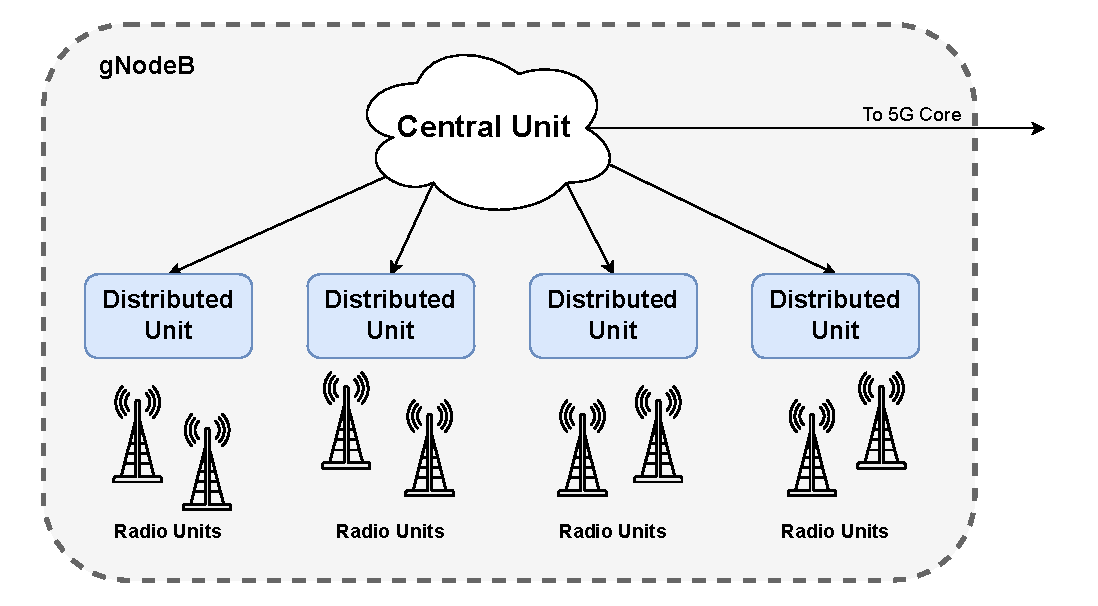
\includegraphics[width=\textwidth]{5G RAN Units.pdf}
  \caption{\gls{gNB} Architecture~\cite{sirotkin2021:5g}}
  \label{fig:5g_ran_architecture}
\end{figure}
% Describe the architecture of the 5G RAN, including key components such as gNodeB, distributed units (DUs), central units (CUs), and their roles in the network, along with the interfaces between them (e.g., F1, NG, Xn).

The architecture of the \gls{NG-RAN} has been fundamentally redesigned to provide higher flexibility by disaggregating the traditional base station functions into more modular components. At its core, the \gls{NG-RAN} is built around the \glsxtrlong{gNB}~(\glsxtrshort{gNB}) (Figure~\ref{fig:5g_ran_architecture}), the 5G equivalent of 4G'S \glsxtrshort{eNB}, responsible for radio transmission, user-plane data forwarding and control-plane signaling with the 5G Core network.

The \gls{gNB} is further divided into three main functional units, which will be described below, with the protocol stack summarized in Figure~\ref{fig:5g_ran_deployment_options}: 
\begin{description}
  \item[\normalfont\uline{\glsxtrlong{CU}}]~\\
  This unit is responsible for higher-layer protocol processing, such as \gls{RRC} and \gls{PDCP}, handling mobility, security and \gls{QoS} flows, and is typically deployed in centralized locations and/or cloud environments. The \gls{CU} can manage multiple \glspl{DU}, coordinating resource usage across a wide area.
  \item[\normalfont\uline{\glsxtrlong{DU}}]~\\
  The \gls{DU} handles lower-layer protocol processing, including \gls{RLC}, \gls{MAC} and \gls{PHY} functions. Multiple of these units can be connected to the same \gls{CU} and they are usually deployed closer to the radio sites to minimize latency and optimize radio resource management.
  \item[\normalfont\uline{\glsxtrlong{RU}}]~\\
  The \glspl{RU} are responsible for the radio frequency functions, including signal transmission and reception, amplification, and antenna management. These are composed of the actual antennas which interact with the \glspl{UE}, along with the necessary back-end, and they are typically located at the cell site. They are connected to the \gls{DU} through front-haul links.
\end{description}
\begin{figure}[H]
  \centering
  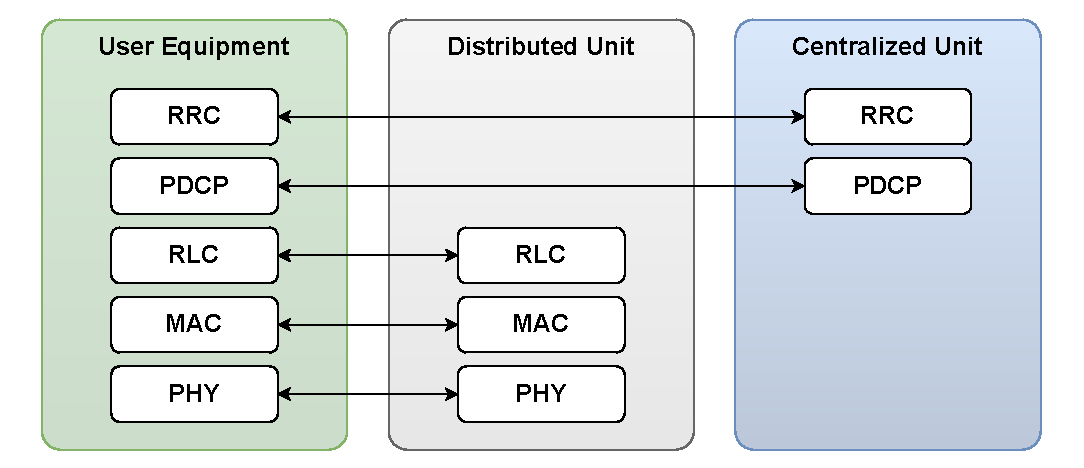
\includegraphics[width=\textwidth]{5G Protocol Stack.pdf}
  \caption{5G RAN Protocol Stack~\cite{sirotkin2021:5g}}
  \label{fig:5g_ran_deployment_options}
\end{figure}
\subsection{RAN Interfaces}
\label{sec:ran_interfaces}
\begin{figure}[H]
  \centering
  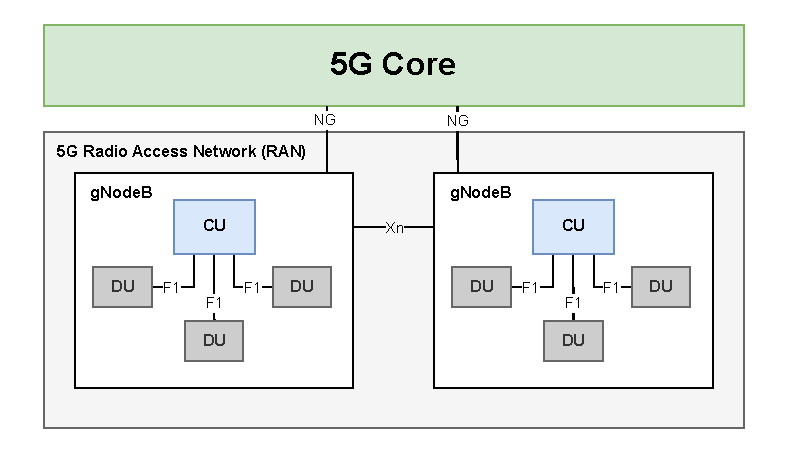
\includegraphics[width=\textwidth]{5G RAN.pdf}
  \caption{5G RAN ~\cite{sirotkin2021:5g}}
  \label{fig:5g_ran_interfaces}
\end{figure}
As depicted in Figure~\ref{fig:5g_ran_interfaces}, the 5G \gls{RAN} incorporates several key interfaces that facilitate communication between its components and with the 5G Core network. The primary interfaces include:
\begin{description}
  \item[\normalfont\uline{NG Interface}]~\\
  The NG interface connects the \gls{gNB} to the 5G Core network. It is further divided into two sub-interfaces: NG-C for control plane signaling and NG-U for user plane data transfer, facilitating both control plane and user plane communications. 
  \item[\normalfont\uline{Xn Interface}]~\\
  The Xn interface connects \glspl{gNB} between each other, enabling inter-cell coordination and handover management. This interface also supports dual connectivity scenarios, where a \gls{UE} can be simultaneously connected to multiple \glspl{gNB} for improved performance and reliability. 
  \item[\normalfont\uline{F1 Interface}]~\\
  The F1 interface connects the \glspl{DU} to the \gls{CU} within the \gls{gNB}. It is also divided into two sub-interfaces: \gls{F1-U} for user plane data and \gls{F1AP} for control plane signaling.
\end{description}
\subsection{RAN Features}
\label{sec:ran_features}
%[Massive MIMO, beamforming and integration with edge computing. Mention frequency ranges FR1/FR2, will be touched upon later]

5G \glsxtrshort{NR} develops upon pre-existing technologies, introduced in previous generations, while introducing new features to meet the ever-demanding requirements of modern mobile communications. One feature that dintinguishes \glsxtrshort{NR} from its predecessors is its \gls{MIMO} technology, introducing Massive \gls{MIMO}.

\begin{figure}[H]
  \centering
  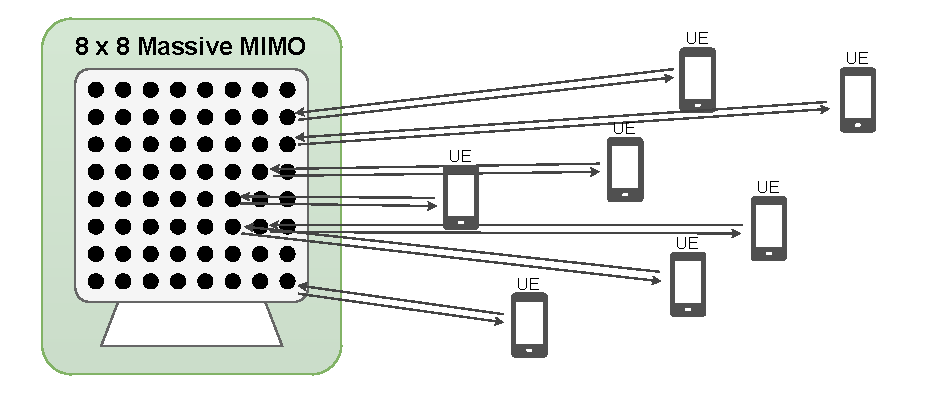
\includegraphics[width=0.8\textwidth]{Massive MIMO.pdf}
  \caption{Massive MIMO antennas}
  \label{fig:5g_ran_features}
\end{figure}

In 4G \glsxtrshort{LTE}, \gls{MIMO} capabilities were already employed, dividing the available antennas between different spatial cells to increase spectral efficiency and throughput. However, 5G \gls{NR} takes this concept further by significantly increasing the number of antennas at the base station, often with upwards of 100+ antennas per \gls{gNB} (Figure~\ref{fig:5g_ran_features}), allowing for \glsxtrlongpl{UE} to be served simultaneously by a single node using the same time-frequency resources. 

Each antenna is capable of beamforming, which focuses the radio signal directly towards the \gls{UE}, rather than broadcasting it omnidirectionally. By dynamically adjusting the phase and amplitude of the signal at each antenna, the system can create highly directional beams that target specific users or cells. This not only improves signal strength and throughput, but also reduces wasted energy and interference with other devices, enhancing the \gls{QoS}.

Driven by the increasing demand for higher bandwidths, \glsxtrshort{3GPP} Release 17~\cite{3GPPRelease17} extended the operation spectrum up to 71 GHz, subdividing the frequency ranges into two categories, as shown in Figure~\ref{fig:5g_frequency_bands}.
\begin{figure}[H]
  \centering
  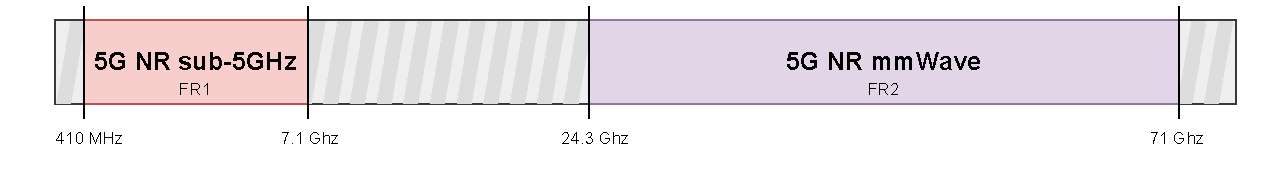
\includegraphics[width=0.95\textwidth]{Frequency Spectrum.pdf}
  \caption{5G Frequency Bands}
  \label{fig:5g_frequency_bands}
\end{figure}
\begin{itemize}
  \item \uline{Frequency Range 1 (FR1)}: Known as the Sub-6GHz range, it encompasses frequencies from 410 MHz to 7.125 GHz. 
  \item \uline{Frequency Range 2 (FR2)}: Known as \glsxtrshort{mmWave}, it covers frequencies from 24.25 GHz to 71 GHz. This range greatly increases available bandwidth and, therefore, throughput, but suffers from significant path loss. It is important to note that many \glsxtrshort{COTS} devices are not compatible with the frequency range.
\end{itemize}
\pagebreak

\section{5G Core}
\label{sec:5g_core}
\begin{figure}[H]
  \centering
  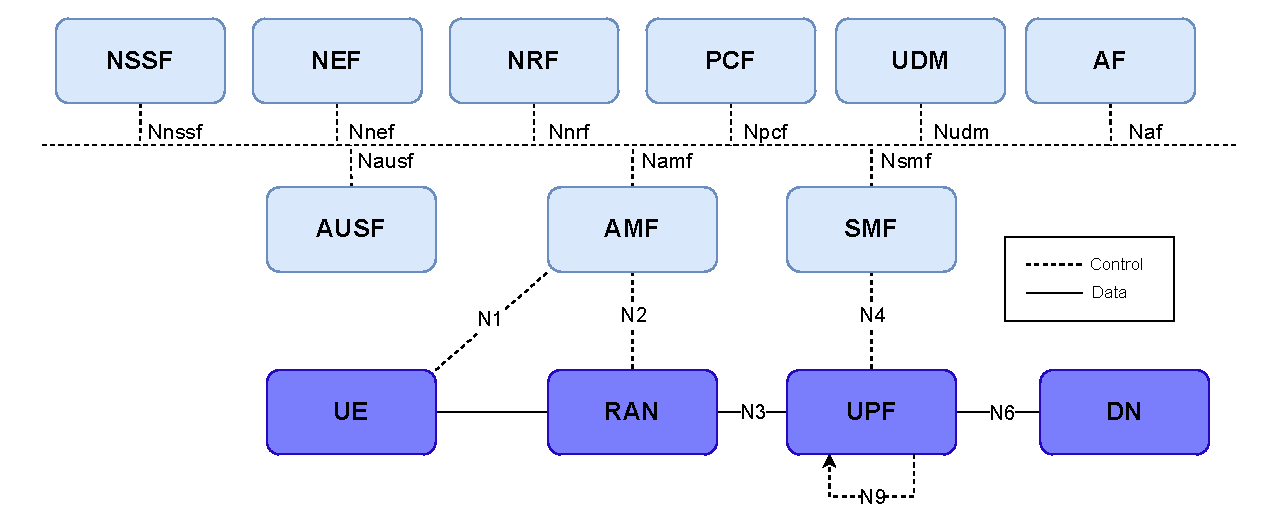
\includegraphics[width=\textwidth]{5G Core.drawio.pdf}
  \caption{5G Core Network Architecture~\cite{sirotkin2021:5g}}
  \label{fig:5g_core_network_architecture}
\end{figure}
As mentioned before [\ref{sec:sba}], a key difference between the 5G Core network and the \gls{EPC} used in 4G networks is the adoption of a service-based architecture. Network Functions are main components that form the 5G Core, and are designed to be modular and communicate with each other using standardized \glspl{API}, allowing for greater flexibility, scalability, and the ability to introduce new services easily.

\subsection{Core Network Functions}
\label{sec:5g_core_network_functions}
As discussed in Section~\ref{sec:CUPS}, \gls{CUPS} defines the separation of control plane and user plane functions. As defined by~\textcite{rommer2020:5g_core_networks}, the main control plane functions are described below:
\subsubsection{Control Plane}
\label{sec:control_plane}

\begin{description}
  \item[\normalfont\uline{\glsxtrlong{AMF}}]~\\
  The \gls{AMF} is a key control plane function in the 5G Core network, counterpart of the \gls{EPC}'s  \gls{MME}. It is responsible for handling connection and mobility management tasks for the \gls{UE}. It manages registration, authentication, reachability, and mobility procedures, ensuring seamless connectivity as users move across different network areas. The AMF also interfaces with other network functions to facilitate session management and policy enforcement.
  
  \item[\normalfont\uline{\glsxtrlong{SMF}}]~\\
  The \gls{SMF} is the function responsible for establishing, modifying and releasing \gls{PDU} sessions, determining the protocol used for communication (IPv4, IPv6, Ethernet, etc), and selecting the \gls{UPF} that will handle the user plane traffic for each session. It also manages IP address allocation for the \gls{UE} and, along with the \gls{PCF}, enforces policies related to session management.

  \item[\normalfont\uline{\glsxtrlong{PCF}}]~\\ 
  Equivalent to \gls{EPC}'s \gls{PCRF}, the \gls{PCF} is responsible for policy control and decision-making within the 5G Core network. Besides this, the \gls{PCF} also has the additional responsibility of providing policy information to the \gls{UE}, such as Access Network Discovery, Selection Policies and UE Route Selection Policies.

  \item[\normalfont\uline{\glsxtrlong{UDM} \& \glsxtrlong{UDR}}]~\\
  The \gls{UDM}, along with the \gls{UDR}, serve as the 5GC equivalent to \gls{EPC}'s \gls{HSS}. These functions are responsible for storing and managing subscriber data and profiles. The \gls{UDR} stores user subscription information, including authentication credentials, service entitlements, and policy data. The \gls{UDM} serves as a front-end to the registry, interacting with other network functions, specifically with the \gls{PCF} and \glsxtrshort{NEF} to facilitate user authentication, authorization, and mobility management.

  \item[\normalfont\uline{\glsxtrlong{NRF}}]~\\ 
  The \glsxtrlong{NRF} is a central component of the 5G Core network that serves as a service registry and discovery function. It maintains a database of available network functions and which services they offer, allowing other network functions to dynamically discover and interact with each other, without the need for them to be configured beforehand. The NRF plays a crucial role in enabling the service-based architecture of the 5G Core, facilitating communication and coordination among various network functions.

  \item[\normalfont\uline{\glsxtrlong{AUSF}}]~\\ 
  The \gls{AUSF} is responsible for handling authentication procedures within the 5G Core network. It works in conjunction with the \gls{UDR}/\gls{UDM} to authenticate \glspl{UE}  attempting to access the network. The \gls{AUSF} is also responsible for providing security parameters in roaming contexts and ensuring that authentication processes comply with 5G security standards. 
  \item[\normalfont\uline{\glsxtrlong{NEF}}]~\\ 
  Equivalent to \gls{EPC}'s \gls{SCEF}, the \gls{NEF} acts as an intermediary between the 5G Core network and external application functions. Network services and events, such as the location of an \gls{UE}, the reachability of the \gls{UE}, its roaming status and loss of connectivity can be exposed by the \gls{NEF} to authorized applications and functions, enabling them to interact with the network in a secure and controlled manner. The \gls{NEF} also handles \glsxtrshort{API} management, security, and policy enforcement for these interactions.
\end{description}
Other more specific control plane functions, such as the \gls{NSSF}, \gls{NWDAF}, \gls{N3IWF}, \gls{AF}, \gls{SMSF} and \gls{LMF} are defined.

\subsubsection{User Plane}
\label{sec:user_plane}
The user plane in the 5G Core network is composed of a single main function, the \glsxtrlong{UPF}. It is responsible for handling all the user data traffic between the \gls{RAN} and external data networks. It performs packet routing and forwarding, \glsxtrshort{QoS} enforcement, traffic shaping, as well as usage reporting and, in some cases, lawful interception. Multiple \glspl{UPF} can be deployed in series, co-existing within the same 5G Core network, enabling distributed architectures and facilitating scalability if necessary. 

\subsection{Core Interfaces}
\label{sec:5gc_interfaces}
Information exchange inside the 5G Core happens through a common access medium using \glspl{API} but, for communication with outside components, it relies on a set of interfaces that define how \glspl{UE}, the \gls{RAN} and the various network functions exchange information. These interfaces are designed to support the service-based architecture of the 5G Core, communicating directly with network functions. The main interfaces, as seen on Figure~\ref{fig:5g_core_network_architecture}, are summarized in Table~\ref{tab:5g_core_network_interfaces}.
\begin{table}[htbp]
  \centering
  \begin{tabular}{|c|c|c|}
    \hline
    \rowcolor{gray!30} 
    \textbf{Interface} & \textbf{Connections} & \textbf{Protocol} \\
    \hline
    N1 & \gls{UE} $\leftrightarrow$ \gls{AMF} & NAS over \glsxtrshort{NG-C} \\
    \hline
    N2 & \gls{RAN} $\leftrightarrow$ \gls{AMF} & \glsxtrshort{NGAP} \\
    \hline
    N3 & \gls{RAN} $\leftrightarrow$ \gls{UPF} & \glsxtrshort{GTP-U} \\
    \hline
    N4 & \gls{SMF} $\leftrightarrow$ \gls{UPF} & \glsxtrshort{GTP-C} \\
    \hline
    N6 & \gls{UPF} $\leftrightarrow$ external \glsxtrshortpl{DN} & IP-based Protocols \\
    \hline
    N9 & \glspl{UPF} $\leftrightarrow$ \glspl{UPF} & \glsxtrshort{GTP-U} \\
    \hline
  \end{tabular}
  \caption{5G Core Network Interfaces~\cites{rommer2020:5g_core_networks}{sirotkin2021:5g}}
  \label{tab:5g_core_network_interfaces}
\end{table}
\section{Existing Open-Source Software for 5G Networks}
\label{sec:existing_5g_packages}
Overall, \gls{OSS} has been a growing tendency in the computer engineering field, and the telecommunications sector is no exception. The adoption of \gls{OSS} for 5G networks has been driven by the need for cost-effective, flexible and customizable solutions that can adapt to the rapidly evolving landscape of mobile communications.

These tools play a crucial role in research, prototyping and, in some cases, even production deployments of 5G networks, as they allow developers to freely experiment with 5G architectures without relying on expensive proprietary solutions. The existing suite of open-source projects already spans both the 5G Core and \gls{RAN}, as well as other tools for support testing, evaluating performance and validation.

\subsection{Open-Source 5G Core Implementations}
\label{sec:open_source_5g_core_implementations}
On the core side, many projects have emerged to provide an accessible way to deploy a complete 5G core network using \gls{OSS} components, with varying levels of maturity. Some of the most notable projects will be described below, with a brief overview on Table~\ref{tab:5gcore_implementations}.

\begin{table}[htbp]
\centering
\footnotesize
\begin{tabularx}{\textwidth}{|l|p{2.2cm}|p{2.1cm}|p{7.5cm}|}
\hline
\rowcolor{gray!30} 
\textbf{Project} & \textbf{Programming Language} & \textbf{Supported Generations} & \textbf{Maturity level}\\ \hline
\textbf{Open5GS} & C & 4G/5G & Most widely adopted open-source 5G Core implementation, with extensive documentation and community support. Used in multiple research projects. \\ \hline
\textbf{Free5GC} & Go & 5G & Well-maintained project with a focus on web-services integration. Less popular than Open5GS but still used in academia.\\ \hline
\textbf{Magma} & C++, Go, Python & 2G/3G/4G/5G & Newer project with a focus on rural connectivity. Growing community and adoption, but less mature than other solutions.\\ \hline
\textbf{\gls{OAI} Core} & C++ & 4G/5G & Backed by major industry players, well-documented and widely used in academia. Container-based deployment for ease of management.\\ \hline
\end{tabularx}
\caption{Overview of different open-source 5G Core implementations.}
\label{tab:5gcore_implementations}
\end{table}

\subsubsection*{\normalfont\uline{Open5GS}}
Open5GS \cite{open5gs_repo} is an open-source implementation of a 5G Core network, written in C language. Out-of-the-box, it provides a set of both 5G Core network functions, such as control plane functions (\gls{AMF}, \gls{SMF}, \gls{PCF}, etc.) and the user plane function (\gls{UPF}), as well as 4G \gls{EPC} functions for \gls{NSA} implementations and backwards compatibility. It focuses on being lightweight and easy to deploy, containing extensive documentation which guides a developer from installation to configuration and, finally, operation. Each network function in Open5GS is defined in a separate configuration file, making it straightforward to modify individual components without affecting the entire system.
Open5GS is one of the most widely adopted open-source 5G Core implementations, as seen in \cites{bonati2025_5gct}{horstmann2025open5gcube}{mamushiane2023deploying}{tio2025exploring5g}, making it a popular choice for research and prototyping of 5G networks.

\subsubsection*{\normalfont\uline{Free5GC}}
\label{sec:free5gc}

Free5GC~\cite{free5gc_repo} is another open-source project that offers an implementation of the 5G Core, written in Go, which integrates well with web-services. It provides a full suite of 5G Core network functions, as according to \glsxtrshort{3GPP} Release 15~\cite{3GPPRelease15}. Although not as popular as other deployments, Free5GC has been used in academia, as seen in \cite{horstmann2025open5gcube}, and has an active community that contributes to its development and maintenance.

\subsubsection*{\normalfont\uline{Magma}}
\label{sec:magma}
Initially developed by Facebook, Magma~\cite{magma_repo} is a project that provides 2G, 3G, 4G and 5G Core network implementations, made open-source in 2019. Despite being relatively new, it has seen a spike in contributors and users, mainly due to being designed from scratch to be implemented in poor, rural areas, where connectivity is scarce. Within their project, they offer a full 5G \gls{SA} Core network implementation, written mainly in C++, Go and Python.

While not as widely adopted as other solutions, due to its novelty and lack of extensive documentation, Magma has been used in research, as seen in~\cite{hasan2023building}.
\subsubsection*{\normalfont\uline{OpenAirInterface Core Network}}
\label{sec:openairinterface}

The OpenAirInterface Software Alliance, composed by major global players (such as Nokia, Vodafone or Ericsson), provides a 5G Core~\cite{oai_core_repo} implementation, mainly maintained by its community. It is written in C++  and provides a complete set of 5G Core network functions, based on containers, making it easy to deploy and manage. The project is well-documented, has many tutorials and examples and has an active community. It is widely used in academia and research, as seen in \cites{bonati2025_5gct}{horstmann2025open5gcube}{vazquez2024maq5g}


\subsection{Open-Source 5G RAN Implementations}
\label{sec:open_source_5g_ran_implementations}
On the \gls{RAN} side, many open-source projects have also emerged to provide 5G \gls{RAN} implementations, but two key players stand out from the rest, srsRAN and OpenAirInterface \gls{RAN}, due to their maturity, extensive documentation and active communities. These projects are described below, with a summarized comparison on Table~\ref{tab:5gran_implementations}.

\begin{table}[htbp]
\centering
\footnotesize
\renewcommand{\arraystretch}{1.5}
\begin{tabularx}{\textwidth}{|l|X|X|}
\hline
\rowcolor{gray!30} 
\textbf{Feature} & \textbf{srsRAN} & \textbf{OpenAirInterface \gls{RAN}} \\ \hline
Frequency Bands Supported & All FR1 (sub-6 GHz) bands & All FR1 and FR2 bands \\ \hline
Deployments supported & NSA and SA & NSA and SA \\ \hline
Duplex Mode & FDD/TDD & FDD/TDD \\ \hline
Sub-Carrier Spacing & 15/30 kHz & 15 and 30 kHz (FR1), 120 kHz (FR2) \\ \hline
Bandwidth (BW) & 10, 20, 40, 80, 100 MHz & 10, 20, 40, 80, 100 MHz \\ \hline
Programming Language & C \& C++ & C \& C++ \\ \hline
Antenna Configuration & SISO & SISO and MIMO \\ \hline
Documentation \& Support & Extensive & Fair \\ \hline
Deployment Complexity & Easier and faster to deploy & Complex to deploy \\ \hline
\end{tabularx}
\caption{Comparison of the open-source 5G RAN projects, as described by \textcite{mamushiane2023deploying}.}
\label{tab:5gran_implementations}
\end{table}

\subsubsection*{\normalfont\uline{srsRAN}}
\label{sec:srsran}

% Mention how srsRAN is a popular choice, how it integrates well with Open5GS, how it supports both 4G and 5G, etc.
srsRAN \cite{srsran_project} is an open-source software suite that provides a complete implementation of the 5G \gls{RAN}, as defined by \gls{3GPP}. It is written in both C and C++ languages and is designed to be modular, allowing the developer to customize both the \gls{CU} and \gls{DU} components of the \gls{gNB} separately. 

It supports all FR1 bands, FDD/TDD modes, all bandwidths up to 100 MHz TDD and 50 MHz FDD, 15/30 kHz subcarrier spacing, 256-QAM modulation, Network Slicing, among other features. srsRAN integrates well with Open5GS and is widely adopted in both academia and industry, as seen in \cites{horstmann2025open5gcube}{mamushiane2023deploying}{tio2025exploring5g}{vazquez2024maq5g}.

The srsRAN project also provides 4G \glsxtrshort{LTE} support through its srsRAN 4G project~\cite{srsran_4g_repo}, allowing for backwards compatibility with existing 4G networks.

\subsubsection*{\normalfont\uline{OpenAirInterface RAN}}
\label{sec:openairinterface_ran}

Along with a Core Network, the OpenAirInterface Software Alliance also provides a 5G RAN implementation~\cite{oai5g_repo}, implementing full \gls{gNB} and \gls{UE} functionalities. Also written in C and C++, it is the most complete 5G open-source RAN stack, supporting both \gls{NSA} and \gls{SA} deployments, monolithic \gls{gNB} as well as disaggregated \gls{CU}/\gls{DU} architectures and FR2 frequency band support. Just like srsRAN, it is widely used in academia, as seen in \cites{bonati2025_5gct}{horstmann2025open5gcube}.



\subsection*{UERANSIM}
\label{sec:ueransim}

UERANSIM~\cite{ueransim_repo} is not a \gls{RAN} implementation, but rather a 5G \gls{UE} and \gls{RAN} simulator, written in C++. It can be used to test 5G Core networks without the need for \glspl{SDR}. It supports both \gls{NSA} and \gls{SA} deployments, and can simulate multiple \glspl{UE} simultaneously. 

\section{Related Works}
\label{sec:related_works}
The deployment of 5G networks using \gls{OSS} has already become an area of research, with many researchers having explored the feasibility of deploying 5G networks using open-source components. Very different approaches have been taken, from small-scale testbeds to complex environments integrated with commercial equipment. In this section, a discuss of some relevant works in this area will be presented, followed by an overview of said works on table~\ref{tab:related_works_comparison}. Most of these works were sourced from srsRAN's Research tab, made available on their website.\bigskip

\textcite{tio2025exploring5g} focused on implementing a complete 5G \gls{SA} network testbed and evaluated its performance using different \glspl{UE}. Their approach consisted of using Open5GS for the 5G Core network and srsRAN for the \gls{RAN}, deployed on USRP X310 and B200 \glspl{SDR}. To evaluate the performance of their testbed, they used srsUE, a 5G \gls{UE} implementation developed by the srsRAN project, \glsxtrlong{COTS} \glspl{UE} and a Sixfab 5G HAT mounted on a Raspberry Pi.
Their results showed that the testbed was able to provide connectivity to the \glspl{UE} and achieve average data rates of up to 68.6 Mbps downlink. Their testbed was also able to connect to the internet and, using Speedtest by Ookla, achieve downlink speeds upwards of 20.1 Mbps. They also performed a series of qualitative tests: package downloads through \texttt{apt}, video streaming on Youtube and video calls between \glspl{UE}, with varying degrees of success.\bigskip

On a similar vein to the previous work, \textcite{vazquez2024maq5g} developed a complete 5G \gls{SA} testbed, named "MAQ5G". Their approach relies solely on the OpenAirInterface project, deploying both their 5G Core and \gls{RAN} software on USRP X310 and B210 \glspl{SDR}, with some modifications to the \gls{gNB} scheduler's code.
Although similar, the evaluation done on this work shines a bigger light on the radio performance, measuring the throughput through different means of transmission and \gls{RAN} configurations, using two \glsxtrshort{COTS} devices outfitted with writable SIM cards. The authors also evaluated the \gls{RAN} host system's performance under different traffic loads, measuring CPU usage.
Results showed that their testbed was able to provide connectivity to the \glspl{UE} and was able to achieve a maximum downlink throughput of 149 Mbps, although they also observed that, under high traffic loads, the host system's behaviour became unreliable, leading to loss of connection for the \glspl{UE}, being the solution a full \gls{UE} reboot.\bigskip

\textcite{mamushiane2023deploying} also developed a 5G \gls{SA} testbed using Open5GS and srsRAN. Their report shines a bigger light on the network development, detailing extensively their configuration decisions and the necessary steps to deploy the network successfully. They also provide a guide for troubleshooting network issues.
While not being the central topic of their work, they evaluated the performance of their testbed, presenting a \gls{gNB} trace showing perfect conditions for the connection, with 0 to 1 packets dropped on downlink and no packets dropped on uplink.\bigskip

Shifting their focus towards containerization, orchestration and the complexity of managing different software stacks, \textcite{horstmann2025open5gcube} developed a complete general-purpose network framework named Open5GCube, able to deploy both 5G \gls{SA} and \gls{NSA} deployments modularly, as well as 4G \glsxtrshort{LTE} and 2G \glsxtrshort{GSM} networks.
Their approach focuses on containerization using Docker Containers, allowing the developers to interchange between different implementations of both the 5G Core and \gls{RAN} components seamlessly. To orchestrate the deployment of the network, they developed their own orchestration script.
Their testbed implements Open5GS, Free5GC and OAI Core as 5G Cores, and srsRAN and OpenAirInterface RAN as \gls{RAN} implementations, built upon two USRP X310 \glspl{SDR} using a 10 MHz \glsxtrshort{GPSDO} for synchronization.
To evaluate their framework, they used several \glsxtrlong{COTS} \glspl{UE}, with different Operating Systems and network chips, and a Quectel RM500Q-GL modem. Results showed that their framework was able to provide 2G and 4G connectivity to all \glspl{UE}, while 5G performance varied between the different \glspl{UE} , with some being able to establish connection seamlessly to the network, while others could only connect to the RAN but not initiate a \glsxtrshort{PDU} session. \bigskip

% 5G-CT
Integrating \glsxtrshort{CD/CI} and automation tools, \textcite{bonati2025_5gct} presented "5G-CT",a framework focused on automated deployment and \gls{OTA} testing. Their network consisted of a Open5GS core, a A5G Networks core and OpenAirInterface \gls{RAN}, deployed at a Northeastern University lab.
Their work stands out due to the tools they employed: OpenShift, a Kubernetes cluster where the Core and \gls{RAN} components would be deployed, and GitOps workflows, the automation tool used to orchestrate the deployment of the network. By using these tools, they automated the provisioning of their 5G networks, effectively streamlining the setup and guaranteeing a consistent and reproducible deployment process.
To demonstrate the capabilities of their framework, they conducted a series of tests over the course of nine months. During this period, the framework executed a daily operation cycle, automatically deploying the network, connecting the \gls{UE} to the network and exchanging UDP traffic between them for 6 hours at varying data rates. In the end, the framework would report the results to another OpenShift pod, where they would be analyzed, and tear down the network.
Results showed that their framework was able to setup the network successfully and tests were ran as planned, presenting little to no packet-loss.\bigskip

%Ericsson RAN
While these works focus on \gls{OSS} implementations using \glspl{SDR}, \textcite{zu2025realworld} bridged the gap between \gls{OSS} and commercial applications, focusing on the realism and the scale of real-world deployments. Their approach consisted on implementing a 5G core using Open5GS along with a proprietary Ericsson \gls{RAN}, deployed on a 30km wireless lab in City of Ames, Iowa.
Their lab was composed of 4 \glspl{gNB} and 30+ \gls{UE} sites equipped with Quectel radios, scattered across residential areas, commercial buildings and farm lands, providing a diverse range of environments to test the network's performance. Results show that their network was able to provide connectivity to all \glspl{UE} and achieve throughput speeds around 320 Mbps, thus proving that an open-source 5G Core can reliably sustain carrier-grade performance and real-world deployments. 

\begin{table}[htbp]
\centering
\footnotesize
\begin{tabularx}{\textwidth}{|p{0.9cm}|p{1.3cm}|p{1.3cm}|p{1.6cm}|X|p{1.5cm}|p{2.3cm}|}
\hline
\rowcolor{gray!30} 
\textbf{Paper} & \textbf{Core} & \textbf{RAN} & \textbf{UE} & \textbf{Containerization} & \textbf{Antenna Config} & \textbf{SDR} \\ \hline
\cite{bonati2025_5gct} & \gls{OAI}, Open5GS, A5G & \gls{OAI} & Sierra Wireless Radio & OpenShift and GitOps workflow & & 8x USRP X310/X410 \\ \hline
\cite{horstmann2025open5gcube} & Open5GS, Free5GC, srsRAN, \gls{OAI} & \gls{OAI}, srsRAN & COTS, Modem & Docker Containers &  & USRP X310 \\ \hline
\cite{mamushiane2023deploying} & Open5GS & srsRAN & COTS, Emulator & OpenStack on Docker Containers & MIMO & NI-2944R \\ \hline
\cite{tio2025exploring5g} & Open5GS & srsRAN & COTS, 5G HAT, Emulator & Docker Containers & MIMO & USRP X310/B200 \\ \hline
\cite{vazquez2024maq5g} & \gls{OAI} & \gls{OAI} & \gls{COTS} & Docker Containers & SISO (custom scheduler) & USRP X310/B210 \\ \hline
\cite{zu2025realworld} & Open5GS & Ericsson & Quectel modem & N/A & Massive MIMO & Ericsson proprietary\\ \hline
\end{tabularx}
\caption{Overview of the network implementations of related works.}
\label{tab:related_works_comparison}
\end{table}